\documentclass[letterpaper,10pt]{article}
\usepackage{mystyle} % This line imports your custom style settings

\begin{document}
\pagestyle{fancy}
\setlength{\headheight}{15pt}
	\begin{flushleft}

\begin{center}
    % Using \textsc for small caps in the author's name can give a nice typographic effect
    % Adjusted the vertical spacing for better visual separation

    {\Large\textbf{How To Prove It:}\\[0.2em] % Bold for the title makes it stand out more
    \Large\textbf{A Structured Approach, Second Edition}}\\[1.5em]

    {\normalsize By \textsc{Daniel J. Velleman}}\\[1.5em]

    % Italicizing "Solutions to" adds emphasis and differentiates from the section title
    Solutions to: \textit{1.4 Operations on Sets}\\[1.5em]

    % "By" is usually not emphasized, normal text is used
    By Cesar Gonzalez\\[0.5em]
    June 2024
\end{center}

\tableofcontents
\newpage

% Sectioning each exercise for TOC
\section*{Exercise 1}
\addcontentsline{toc}{section}{Exercise 1}
% This is exercise.tex
% Ex 1
\begin{enumerate}[label=(\alph*)]
    \item Factor $2^{15}-1=32,767$ into a product of two smaller positive integers.
    \item Find an integer $x$ such that $1<x<2^{32767}-1$ and $2^{32767}-1$ is divisible by $x$.
\end{enumerate}

\textbf{Solution:}
\begin{enumerate}[label=(\alph*)]
   \item From the \textit{Proof of Conjecture 2}, we are given that
   $$xy=(2^b-1)(1+2^b+2^{2b}+2^{3b}+...+2^{(a-1)(b)})=2^{ab}-1=2^n-1$$
   where $n$ is not prime, $x$ is not prime, $y$ is not prime, and $n,x,y,a,b$ are all positive integers. If $n=15$, then let $a=3$ and $b=5$. Hence, 
   \begin{align*}
       2^{15}-1 &= 2^{(3)(5)}-1 \\
       &= (2^5-1)(1+2^5+2^{(3-1)(5)})\\
       &= (32-1)(1+32+2^{10})\\
       &= (31)(33+1024)\\
       &= (31)(1057)\\
       &= 32767
   \end{align*}
   We have thus factored $32,767$ as a product of $31$ and $1057$.

   \item Similarly as with (a), if $n=32767$, then let $a=31$ and $b=1057$. Hence, 
   \begin{align*}
       2^{32767}-1 &= 2^{(31)(1057)}-1 \\
       &= (2^{31}-1)(1+2^{31}+2^{2(31)}+2^{3(31)}+...+2^{(1057-1)(31)})\\
       &= (2^{31}-1)(1+2^{31}+2^{2(31)}+...+2^{(1056)(31)})
   \end{align*}
   where $x=2^{31}-1$ and $y=1+2^{31}+2^{2(31)}+...+2^{(1056)(31)}$. We know from the \textit{Proof of Conjecture 2} that both $x,y$ are positive integers each smaller than $n$. Either can serve as the solution to the problem. For example, $x$ is greater than one and less than $2^{32767}-1$, and $x$ divides $2^{32767}-1$.
\end{enumerate}

\pagebreak

\section*{Exercise 2}
\addcontentsline{toc}{section}{Exercise 2}
Make truth tables for the following formulas:
\begin{enumerate}[label=(\alph*)]
    \item $\neg [P \wedge (Q \vee \neg P)]$.
    \item $(P \vee Q) \wedge (\neg P \vee R).$
\end{enumerate}

\textbf{Solution:}
\begin{enumerate}[label=(\alph*)]
\item 
\[
\begin{array}{|c|c|c|c|c|c|}
\hline
P & Q & \neg P & Q \vee \neg P & P \wedge (Q \vee \neg P) & \neg [P \wedge (Q \vee \neg P)] \\
\hline
\text{False} & \text{False} & \text{True} & \text{True} & \text{False} & \text{True} \\
\text{False} & \text{True} & \text{True} & \text{True} & \text{False} & \text{True} \\
\text{True} & \text{False} & \text{False} & \text{False} & \text{False} & \text{True} \\
\text{True} & \text{True} & \text{False} & \text{True} & \text{True} & \text{False} \\
\hline
\end{array}
\]

\item
\[
\begin{array}{|c|c|c|c|c|c|c|}
\hline
P & Q & R & \neg P & P \vee Q & \neg P \vee R & (P \vee Q) \wedge (\neg P \vee R) \\
\hline
\text{False} & \text{False} & \text{False} & \text{True} & \text{False} & \text{True} & \text{False} \\
\text{False} & \text{False} & \text{True} & \text{True} & \text{False} & \text{True} & \text{False} \\
\text{False} & \text{True} & \text{False} & \text{True} & \text{True} & \text{True} & \text{True} \\
\text{True} & \text{False} & \text{False} & \text{False} & \text{True} & \text{False} & \text{False} \\
\text{False} & \text{True} & \text{True} & \text{True} & \text{True} & \text{True} & \text{True} \\
\text{True} & \text{False} & \text{True} & \text{False} & \text{True} & \text{True} & \text{True} \\
\text{True} & \text{True} & \text{False} & \text{False} & \text{True} & \text{False} & \text{False} \\
\text{True} & \text{True} & \text{True} & \text{False} & \text{True} & \text{True} & \text{True} \\
\hline
\end{array}
\]
\end{enumerate}

\pagebreak

\section*{Exercise 3}
\addcontentsline{toc}{section}{Exercise 3}
% This is exercise.tex
% Ex 3
The proof of Theorem 3 gives a method for finding a prime number different from any in a given list of prime numbers.

\begin{enumerate}[label=(\alph*)]
    \item Use this method to find a prime different from 2,3,5, and 7.
    \item Use this method to find a prime different from 2,5, and 11.
\end{enumerate}

\textbf{Solution:}
Recall that \textbf{Theorem 3} gave the following method for finding a prime number different from those in the given list of prime numbers in its premise. If $m=p_1p_2\cdot \cdot \cdot p_n+1$, where $p_1,p_2,..., p_n$ is a list of prime numbers and $m$ is a positive integer, then $m$ is a prime or a product of primes.
\begin{enumerate}[label=(\alph*)]
   \item If $p_1p_2\cdot \cdot \cdot p_n = (2)(3)(5)(7) $, then $m=(2)(3)(5)(7)+1=211$. Note that 211 is prime and not in the list.
   \item If $p_1p_2\cdot \cdot \cdot p_n = (2)(5)(11) $, then $m=(2)(5)(11)+1=111=(3)(37)$. Note that 3 and 37 are prime and not in the list.
\end{enumerate}

\pagebreak

\section*{Exercise 4}
\addcontentsline{toc}{section}{Exercise 4}
% This is exercise.tex
% Ex 4
Find 5 consecutive integers that are not prime.

\doublespacing

\textbf{Solution:} Recall that \textbf{Theorem 4} states that for every positive integer $n$, there is a sequence of $n$ consecutive positive integers containing no primes. More over, if $n$ is a positive integer, and $x=(n+1)!+2$, then $x,x+1,x+2,...,x+(n-1)$ are not prime. Take $n=5$, then
\begin{align*}
    x   &= 6!+2 = 720 + 2 = 722=(2)(361)\\
    x+1 &= 6!+3 = 720 + 3 = 723=(3)(241)\\
    x+2 &= 6!+4 = 720 + 4 = 724=(2)(362)\\
    x+3 &= 6!+5 = 720 + 5 = 725=(5)(145)\\
    x+4 &= 6!+6 = 720 + 6 = 726=(2)(363)
\end{align*}

We have thus found 5 consecutive integers that are not prime.

\pagebreak

\section*{Exercise 5}
\addcontentsline{toc}{section}{Exercise 5}
\begin{enumerate}[label=(\alph*)]
    \item Show that $P \leftrightarrow Q$ is equivalent to $(P \wedge Q) \vee (\neg P \wedge \neg Q)$.
    \item Show that $(P \rightarrow Q) \vee (P \rightarrow R)$ is equivalent to $P \rightarrow (Q \vee R)$.
\end{enumerate}
\textbf{Solution:}
\begin{enumerate}[label=(\alph*)]
    \item Below we prove that $P \leftrightarrow Q \equiv (P \wedge Q) \vee (\neg P \wedge \neg Q)$.
    \begin{alignat*}{2}
        (P \wedge Q) \vee (\neg P \wedge \neg Q) &\equiv [(P \wedge Q) \vee \neg P] \wedge [(P \wedge Q) \vee \neg Q] && \quad \textbf{Distributive Law}\\
        &\equiv [(P \vee \neg P) \wedge (Q \vee \neg P)] \wedge [(P \vee \neg Q) \wedge (Q \vee \neg Q)] && \quad \textbf{Distributive Law}\\
        &\equiv [\text{Tautology} \wedge (Q \vee \neg P)] \wedge [(P \vee \neg Q) \wedge \text{Tautology}] && \quad \textbf{Def. of Tautology}\\
        &\equiv (Q \vee \neg P) \wedge (P \vee \neg Q) && \quad \textbf{Law of Tautology}\\
        &\equiv (\neg P \vee Q) \wedge (\neg Q \vee P) && \quad \textbf{Commutative Law}\\
        &\equiv (P \rightarrow Q) \wedge (Q \rightarrow P) && \quad \textbf{Conditional Law}\\
        &\equiv P \leftrightarrow Q && \quad \textbf{Biconditional Law}\\
    \end{alignat*}
    
    \item Below we prove that $(P \rightarrow Q) \vee (P \rightarrow R) \equiv P \rightarrow (Q \vee R)$.
    \begin{alignat*}{2}
        (P \rightarrow Q) \vee (P \rightarrow R) &\equiv (\neg P \vee Q) \vee (\neg P \vee R) && \quad \textbf{Conditional Law}\\
        &\equiv \neg P \vee Q \vee \neg P \vee R && \quad \textbf{Associative Law}\\
        &\equiv \neg P \vee \neg P \vee Q \vee R && \quad \textbf{Commutative Law}\\
        &\equiv (\neg P \vee \neg P) \vee (Q \vee R) && \quad \textbf{Associative Law}\\
        &\equiv \neg P \vee (Q \vee R) && \quad \textbf{Idempotent Law}\\
        &\equiv P \rightarrow (Q \vee R) && \quad \textbf{Conditional Law}\\
    \end{alignat*}
\end{enumerate}
\pagebreak

\section*{Exercise 6}
\addcontentsline{toc}{section}{Exercise 6}
Some mathematicians write $P | Q$ to mean "$P$ and $Q$ are not both true". This connective is called \textit{nand}, and is used in the study of circuits in computer science.
\begin{enumerate}[label=(\alph*)]
\item Make a truth table for $P | Q$.
\item Find a formula using only the connectives $\wedge$, $\vee$, and $\neg$ that is equivalent to $P | Q$.
\item Find formulas using only the connective $|$ that are equivalent to $\neg P$, $P \vee Q$, and $P \wedge Q$.
\end{enumerate}

\textbf{Solution:}
\begin{enumerate}[label=(\alph*)]
\item 
\[
\begin{array}{|c|c|c|}
\hline
P & Q & P | Q \\
\hline
\text{False} & \text{False} & \text{True} \\
\text{False} & \text{True} & \text{True} \\
\text{True} & \text{False} & \text{True} \\
\text{True} & \text{True} & \text{False} \\
\hline
\end{array}
\]

\item The formula $\neg (P \wedge Q)$ is equivalent to $P | Q$ since for every possible combination of truth values for the propositions, the truth values of both formulas are the same. 

\[
\begin{array}{|c|c|c|c||c|}
\hline
P & Q & P \wedge Q & \neg (P \wedge Q) & P | Q \\
\hline
\text{False} & \text{False} & \text{False} & \text{True} & \text{True} \\
\text{False} & \text{True} & \text{False} & \text{True} & \text{True} \\
\text{True} & \text{False} & \text{False} & \text{True} & \text{True} \\
\text{True} & \text{True} & \text{True} & \text{False} & \text{False} \\
\hline
\end{array}
\]

\pagebreak

\item \begin{itemize}
    \item The formula $P | P$ is equivalent to $\neg P$.
    \[
    \begin{array}{|c|c|c||c|}
    \hline
    P & P & P | P & \neg P \\
    \hline
    \text{False} & \text{False} & \text{True} & \text{True}\\
    \text{True} & \text{True} & \text{False} & \text{False} \\
    \hline
    \end{array}
    \]

    \item The formula $(P | Q) | (P | Q)$ is equivalent to $\neg (P | Q)$ (using the result from above, i.e., $\neg P \equiv P | P$), hence equivalent to $P \wedge Q$. We justify the answer with our truth table.
    \[
    \begin{array}{|c|c|c|c||c|}
    \hline
    P & Q & P | Q & \neg (P | Q) & P \wedge Q \\
    \hline
    \text{False} & \text{False} & \text{True} & \text{False} & \text{False}\\
    \text{False} & \text{True} & \text{True} & \text{False} & \text{False} \\
    \text{True} & \text{False} & \text{True} & \text{False} & \text{False} \\
    \text{True} & \text{True} & \text{False} & \text{True} & \text{True} \\
    \hline
    \end{array}
    \]

    \item The formula $(P | P) | (Q | Q)$ is equivalent to $P \vee Q$.
    \begin{alignat*}{2}
        P \vee Q & \equiv \neg \neg P \vee \neg \neg Q && \quad \text{(Double Negation Law)} \\
                   & \equiv \neg (\neg P \wedge \neg Q) && \quad \text{(DeMorgan's Law)} \\
                   & \equiv \neg \neg (\neg P | \neg Q) && \quad \text{(Results Above: $\neg(P | Q) \equiv P \wedge Q$)} \\
                   & \equiv \neg P | \neg Q && \quad \text{(Double Negation Law)} \\
                   & \equiv (P | P) | (Q | Q) && \quad \text{(Results Above: $\neg P \equiv P | P$)}
    \end{alignat*}
    We also justify our answer with a truth table.
    \[
    \begin{array}{|c|c|c|c|c||c|}
    \hline
    P & Q & P | P & Q | Q & (P | P) | (Q | Q) & P \vee Q \\
    \hline
    \text{True} & \text{True} & \text{False} & \text{False} & \text{True} & \text{True} \\
    \text{True} & \text{False} & \text{False} & \text{True} & \text{True} & \text{True} \\
    \text{False} & \text{True} & \text{True} & \text{False} & \text{True} & \text{True} \\      
    \text{False} & \text{False} & \text{True} & \text{True} & \text{False} & \text{False} \\
    \hline
    \end{array}
    \]
\end{itemize}
\end{enumerate}

\pagebreak

\section*{Exercise 7}
\addcontentsline{toc}{section}{Exercise 7}
\begin{enumerate}[label=(\alph*)]
    \item Show that $(P \rightarrow Q) \wedge (Q \rightarrow R)$ is equivalent to $(P \rightarrow R) \wedge [(P \leftrightarrow Q) \vee (R \leftrightarrow Q)]$.
    \item Show that $(P \rightarrow Q) \vee (Q \rightarrow R)$ is a tautology.
\end{enumerate}
\textbf{Solution:}
\begin{enumerate}[label=(\alph*)]
    \item Below we prove that $(P \rightarrow Q) \wedge (Q \rightarrow R) \equiv (P \rightarrow R) \wedge [(P \leftrightarrow Q) \vee (R \leftrightarrow Q)]$.\\

    \
    
    First we prove \textbf{Lemma 7.a.1}: $(P \rightarrow Q) \wedge (Q \rightarrow R) \equiv [P \rightarrow (Q \wedge R)] \wedge (Q \rightarrow R)$.
    \begin{alignat*}{2}
        (P \rightarrow Q) \wedge (Q \rightarrow R) &\equiv (\neg P \vee Q) \wedge (\neg Q \vee R) && \quad \textbf{Conditional Law}\\
        &\equiv [(\neg P \vee Q) \wedge \neg Q ]\vee [(\neg P \vee Q) \wedge R] && \quad \textbf{Distributive Law}\\
        &\equiv [(\neg P \wedge \neg Q) \vee (Q \wedge \neg Q)]\vee [(\neg P \wedge R) \vee (Q \wedge R)] && \quad \textbf{Distributive Law}\\
        &\equiv [(\neg P \wedge \neg Q) \vee \text{Contradiction}]\vee [(\neg P \wedge R) \vee (Q \wedge R)] && \quad \textbf{Def. of Contradiction}\\
        &\equiv [\neg P \wedge \neg Q]\vee [(\neg P \wedge R) \vee (Q \wedge R)] && \quad \textbf{Law of Contradiction}\\
        &\equiv (\neg P \wedge \neg Q) \vee (\neg P \wedge R) \vee (Q \wedge R) && \quad \textbf{Associtive Law}\\
        &\equiv [(\neg P \wedge \neg Q) \vee (\neg P \wedge R)] \vee (Q \wedge R) && \quad \textbf{Associtive Law}\\
        &\equiv [\neg P \wedge (\neg Q \vee R)] \vee (Q \wedge R) && \quad \textbf{Distributive Law}\\
        &\equiv [\neg P \vee (Q \wedge R)] \wedge [(\neg Q \vee R) \vee (Q \wedge R)] && \quad \textbf{Distributive Law}\\
        &\equiv [\neg P \vee (Q \wedge R)] \wedge \{[(\neg Q \vee R) \vee Q] \wedge [(\neg Q \vee R) \vee R]\} && \quad \textbf{Distributive Law}\\
        &\equiv [\neg P \vee (Q \wedge R)] \wedge \{[(\neg Q \vee Q) \vee R] \wedge [\neg Q \vee (R \vee R)]\} && \quad \textbf{Associative/Commutative Laws}\\
        &\equiv [\neg P \vee (Q \wedge R)] \wedge \{[(\neg Q \vee Q) \vee R] \wedge (\neg Q \vee R)\} && \quad \textbf{Idempotent Law}\\
        &\equiv [\neg P \vee (Q \wedge R)] \wedge \{[\text{Tautology} \vee R] \wedge (\neg Q \vee R)\} && \quad \textbf{Def. of Tautology}\\
        &\equiv [\neg P \vee (Q \wedge R)] \wedge [\text{Tautology} \wedge (\neg Q \vee R)] && \quad \textbf{Law of Tautology}\\
        &\equiv [\neg P \vee (Q \wedge R)] \wedge (\neg Q \vee R) && \quad \textbf{Law of Tautology}\\
        &\equiv [P \rightarrow (Q \wedge R)] \wedge (Q \rightarrow R) && \quad \textbf{Conditional Law}\\
    \end{alignat*}
    We also prove \textbf{Lemma 7.a.2}: $(P \rightarrow Q) \wedge (P \rightarrow R) \equiv [P \rightarrow (Q \wedge R)]$.
    \begin{alignat*}{2}
        (P \rightarrow Q) \wedge (P \rightarrow R) &\equiv (\neg P \vee Q) \wedge (\neg P \vee R) && \quad \textbf{Conditional law}\\
        &\equiv \neg P \vee (Q \wedge R) && \quad \textbf{Distributive law}\\
        &\equiv P \rightarrow (Q \wedge R) && \quad \textbf{Conditional law}\\
    \end{alignat*}
    We also prove \textbf{Lemma 7.a.3}: $Q \rightarrow Q \equiv \text{Tautology}$.
    \begin{alignat*}{2}
        Q \rightarrow Q &\equiv \neg Q \vee Q && \quad \textbf{Conditional law}\\
        &\equiv \text{Tautology} && \quad \textbf{Definition of Tautology}\\
    \end{alignat*}
    \pagebreak

    Proof of \textbf{7.a}:
    \begin{alignat*}{2}
        &(P \rightarrow R) \wedge [(P \leftrightarrow Q) \vee (R \leftrightarrow Q)] && \quad \textbf{RHS}\\
        &\equiv (P \rightarrow R) \wedge \{[(P \wedge Q) \vee (\neg P \wedge \neg Q)] \vee [(R \wedge Q) \vee (\neg R \wedge \neg Q)]\} && \quad \textbf{Exercise 5.a}\\
        &\equiv (P \rightarrow R) \wedge \{[(P \wedge Q) \vee (R \wedge Q)] \vee [(\neg P \wedge \neg Q) \vee (\neg R \wedge \neg Q)]\} && \quad \textbf{Associative/Commutative Laws}\\
        &\equiv (P \rightarrow R) \wedge \{[(P \vee R) \wedge Q] \vee [(\neg P \vee \neg R) \wedge \neg Q]\} && \quad \textbf{Distributive Law}\\
        &\equiv \{(P \rightarrow R) \wedge [(P \vee R) \wedge Q]\} \vee \{(P \rightarrow R) \wedge [(\neg P \vee \neg R) \wedge \neg Q]\} && \quad \textbf{Distributive Law}\\
        &\equiv [(P \rightarrow R) \wedge (P \vee R) \wedge Q] \vee [(P \rightarrow R) \wedge (\neg P \vee \neg R) \wedge \neg Q] && \quad \textbf{Associative Law}\\
        &\equiv [(\neg P \vee R) \wedge (P \vee R) \wedge Q] \vee [(\neg P \vee R) \wedge (\neg P \vee \neg R) \wedge \neg Q] && \quad \textbf{Conditional Law}\\
        &\equiv [\{(\neg P \vee R) \wedge (P \vee R)\} \wedge Q] \vee [\{(\neg P \vee R) \wedge (\neg P \vee \neg R)\} \wedge \neg Q] && \quad \textbf{Associative Law}\\
        &\equiv [\{(\neg P \wedge P) \vee R)\} \wedge Q] \vee [\{\neg P \vee (R \wedge \neg R)\} \wedge \neg Q] && \quad \textbf{Distributive Law}\\
        &\equiv [\{\text{Contradiction} \vee R)\} \wedge Q] \vee [\{\neg P \vee \text{Contradiction}\} \wedge \neg Q] && \quad \textbf{Def. of Contradiction}\\
        &\equiv [R \wedge Q] \vee [\neg P \wedge \neg Q] && \quad \textbf{Law of Contradiction}\\
        &\equiv [(R \wedge Q) \vee \neg P] \wedge [(R \wedge Q) \vee \neg Q] && \quad \textbf{Distributive Law}\\
        &\equiv [\neg P \vee (R \wedge Q)] \wedge [\neg Q \vee (R \wedge Q)] && \quad \textbf{Commutative Law}\\
        &\equiv [P \rightarrow (R \wedge Q)] \wedge [Q \rightarrow (R \wedge Q)] && \quad \textbf{Conditional Law}\\
        &\equiv [(P \rightarrow R) \wedge (P \rightarrow Q)] \wedge [(Q \rightarrow R) \wedge (Q \rightarrow Q)] && \quad \textbf{Lemma 7.a.2}\\
        &\equiv [(P \rightarrow R) \wedge (P \rightarrow Q)] \wedge [(Q \rightarrow R) \wedge \text{Tautology}] && \quad \textbf{Lemma 7.a.3}\\
        &\equiv [(P \rightarrow R) \wedge (P \rightarrow Q)] \wedge (Q \rightarrow R) && \quad \textbf{Law of Tautology}\\
        &\equiv [P \rightarrow (R \wedge Q)] \wedge (Q \rightarrow R) && \quad \textbf{Lemma 7.a.2}\\
        &\equiv (P \rightarrow Q) \wedge (Q \rightarrow R) && \quad \textbf{Lemma 7.a.1}\\
    \end{alignat*}

    \item We prove that $(P \rightarrow Q) \vee (Q \rightarrow R) \equiv \text{Tautology}$.
    \begin{alignat*}{2}
        (P \rightarrow Q) \vee (Q \rightarrow R) &\equiv (\neg P \vee Q) \vee (\neg Q \vee R) && \quad \textbf{Conditional Law}\\
        &\equiv \neg P \vee Q \vee \neg Q \vee R && \quad \textbf{Associative Law}\\
        &\equiv \neg P \vee (Q \vee \neg Q) \vee R && \quad \textbf{Associative Law}\\
        &\equiv \neg P \vee \text{Tautology} \vee R && \quad \textbf{Def. of Tautology}\\
        &\equiv \text{Tautology} \vee \neg P \vee R && \quad \textbf{Commutative Law}\\
        &\equiv \text{Tautology} \vee (\neg P \vee R) && \quad \textbf{Associative Law}\\
        &\equiv \text{Tautology} && \quad \textbf{Tautology Law}\\
    \end{alignat*}
\end{enumerate}
\pagebreak


\section*{Exercise 8}
\addcontentsline{toc}{section}{Exercise 8}
What are the truth sets of the following statements? List a few elements of the truth set if you can.

\begin{enumerate}[label=(\alph*)]
    \item $x$ is a real number and $x^2-4x+3=0$.
    \item $x$ is a real number and $x^2-2x+3=0$.
    \item $x$ is a real number and $5 \in \{y \in \mathbb{R} \ | \ x^2+y^2 < 50 \}$.
\end{enumerate}

\textbf{Solution:}
\begin{enumerate}[label=(\alph*)]
    \item To find the truth set, we need to solve the equation $x^2-4x+3=0$. Using the quadratic formula, we get:
    \begin{align*}
        x &= \frac{-b \pm \sqrt{b^2-4ac}}{2a} \\
          &= \frac{4 \pm \sqrt{(-4)^2-4(1)(3)}}{2(1)} \\
          &= \frac{4 \pm \sqrt{4}}{2} \\
          &= \frac{4 \pm 2}{2} \\
          &= 1 \text{ or } 3
    \end{align*}
    Therefore, the truth set is:
    \begin{align*}
        \{ x \ | \ &x \text{ is a real number and } x^2-4x+3=0 \} \\
        &\equiv \{1, 3\}
    \end{align*}
    
    \item Similarly, solving the equation $x^2-2x+3=0$ using the quadratic formula:
    \begin{align*}
        x &= \frac{-b \pm \sqrt{b^2-4ac}}{2a} \\
          &= \frac{2 \pm \sqrt{(-2)^2-4(1)(3)}}{2(1)} \\
          &= \frac{2 \pm \sqrt{-8}}{2}
    \end{align*}
    Since $\sqrt{-8}$ is not a real number, there are no real solutions to this equation. Therefore, the truth set is:
    \begin{align*}
        \{ x \ | \ &x \text{ is a real number and } x^2-2x+3=0 \} \\
        &\equiv \{\}
    \end{align*}
    
    \item The statement "$5 \in \{y \in \mathbb{R} \ | \ x^2+y^2 < 50 \}$" is equivalent to "$x^2+5^2 < 50$". Solving this inequality:
    \begin{align*}
        x^2+5^2 &< 50 \\
        x^2+25 &< 50 \\
        x^2 &< 25 \\
        -5 < x &< 5
    \end{align*}
    Therefore, the truth set is:
    \begin{align*}
        \{ x \ | \ &x \text{ is a real number and } 5 \in \{y \in \mathbb{R} \ | \ x^2+y^2 < 50 \} \} \\
        &\equiv \{ x \ | \ x \in \mathbb{R} \text{ and } -5 < x < 5 \}
    \end{align*}
    Some elements of this truth set include -4.9, 0, 3.14, etc.
\end{enumerate}

\section*{Exercise 9}
\addcontentsline{toc}{section}{Exercise 9}
It was shown in this section that for any sets $A$ and $B$, $(A \cup B) \mybackslash B \subseteq A$. Give an example of two sets $A$ and $B$ for which $(A \cup B) \mybackslash B \neq A$.

\textbf{Solution:} Suppose $A = \{ 1,2,3,4\}$ and $B = \{4,5,6,7\}$, then $A \cup B = \{1,2,3,4,5,6,7\}$.
Hence, $(A \cup B) \mybackslash B = \{1,2,3\} \not\equiv \{1,2,3,4 \} = A$.
\pagebreak

\section*{Exercise 10}
\addcontentsline{toc}{section}{Exercise 10}
Use truth tables to check these laws:
\begin{enumerate}[label=(\alph*)]
    \item The second DeMorgan's law.
    \item The distributive laws.
\end{enumerate}

\textbf{Solution:}
\begin{enumerate}[label=(\alph*)]
    \item Observe that the truth values are identical for both formulas.
    
\[
\begin{array}{|cc||c|c|}
\hline
P & Q & \neg (P \vee Q) & \neg P \wedge \neg Q\\
\hline
F & F & T & T \\
F & T & F & F \\
F & T & F & F \\
T & T & F & F \\
\hline
\end{array}
\]

\item Observe that the truth values are identical for each pair of formulas.
\[
\begin{array}{|ccc||c|c|}
\hline
P & Q & R & P \wedge (Q \vee R) & (P \wedge Q) \vee (P \wedge R) \\
\hline
F & F & F & F & F \\
F & F & T & F & F \\
F & T & F & F & F \\
F & T & T & F & F \\
T & F & F & F & F \\
T & F & T & T & T \\
T & T & F & T & T \\
T & T & T & T & T \\
\hline
\end{array}
\]

\

\[
\begin{array}{|ccc||c|c|}
\hline
P & Q & R & P \vee (Q \wedge R) & (P \vee Q) \wedge (P \vee R) \\
\hline
F & F & F & F & F \\
F & F & T & F & F \\
F & T & F & F & F \\
F & T & T & T & T \\
T & F & F & T & T \\
T & F & T & T & T \\
T & T & F & T & T \\
T & T & T & T & T \\
\hline
\end{array}
\]
\end{enumerate}

\pagebreak

\section*{Exercise 11}
\addcontentsline{toc}{section}{Exercise 11}
\begin{enumerate}[label=(\alph*)]
    \item Make a Venn diagram for the sets $(A \cup B) \mybackslash C$ and $A \cup (B \mybackslash C)$. What can you conclude about whether one of these sets is necessarily, a subset of the other?
    \item Give an example of sets $A,B,$ and $C$ for which $(A \cup B) \mybackslash C \neq A \cup (B \mybackslash C)$.
\end{enumerate}

\textbf{Solution:}
\begin{enumerate}[label=(\alph*)]
    \item We first draw $A \cup (B \mybackslash C)$ below. \\
    
    \
    
        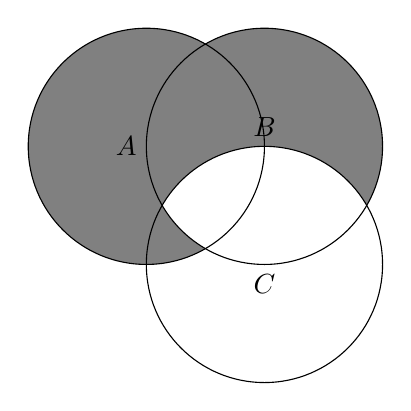
\begin{tikzpicture}
          % Define circles for A, B, and C
          \def\circleA{(0,0) circle (1.5cm)}
          \def\circleB{(1.5,0) circle (1.5cm)}
          \def\circleC{(1.5,-1.5) circle (1.5cm)}
        
          % Fill A
          \begin{scope}
            \fill[gray] \circleA;
          \end{scope}
        
          % Fill B excluding C
          \begin{scope}
            \clip \circleB;
            \fill[gray] \circleB;
            \clip \circleC;
            \fill[white] \circleB;
          \end{scope}
        
          % Outline the circles and label them
          \draw \circleA node [text=black, left] {$A$};
          \draw \circleB node [text=black, above] {$B$};
          \draw \circleC node [text=black, below] {$C$};
        \end{tikzpicture}

    Next, we draw $(A \cup B) \mybackslash C$ below. \\
    
    \
    
        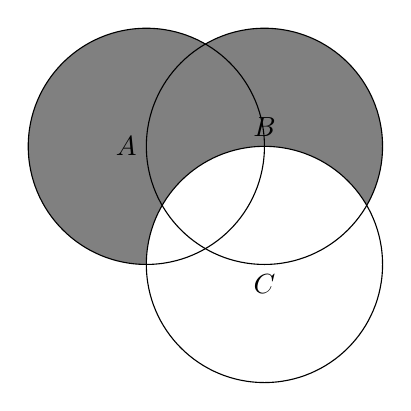
\begin{tikzpicture}
          % Define circles for A, B, and C
          \def\circleA{(0,0) circle (1.5cm)}
          \def\circleB{(1.5,0) circle (1.5cm)}
          \def\circleC{(1.5,-1.5) circle (1.5cm)}
        
          % Fill A
          \begin{scope}
            \fill[gray] \circleA;
            \clip \circleC;
            \fill[white] \circleC;
          \end{scope}
        
          % Fill B excluding C
          \begin{scope}
            \clip \circleB;
            \fill[gray] \circleB;
            \clip \circleC;
            \fill[white] \circleB;
          \end{scope}
        
          % Outline the circles and label them
          \draw \circleA node [text=black, left] {$A$};
          \draw \circleB node [text=black, above] {$B$};
          \draw \circleC node [text=black, below] {$C$};
        \end{tikzpicture}

    Note that in $A \cup (B \mybackslash C)$, $A \cap C$ is nonempty. Meanwhile in $(A \cup B) \mybackslash C$ the set $A \cap C$ is empty. Everything else is equivalent. Hence, $(A \cup B) \mybackslash C \subseteq A \cup (B \mybackslash C)$.
    
    \item Let $A=\{1,2,3\}$, $B=\{3,4,5\}$ and $C=\{1,5\}$. Now, $(A \cup B) \setminus C$ gives us $\{1, 2, 3, 4, 5\} \setminus \{1, 5\} = \{2, 3, 4\}$, while $A \cup (B \setminus C)$ gives us $\{1, 2, 3\} \cup \{3, 4\} = \{1, 2, 3, 4\}$. These two results are clearly different: $\{2, 3, 4\} \neq \{1, 2, 3, 4\}$. This example correctly illustrates the inequality between $(A \cup B) \setminus C$ and $A \cup (B \setminus C)$.
\end{enumerate}
\pagebreak

\section*{Exercise 12}
\addcontentsline{toc}{section}{Exercise 12}
Use Venn diagrams to show that the associative law holds for symmetric difference; that is, for any sets $A$, $B$, and $C$, $A \triangle (B \triangle C) = (A \triangle B) \triangle C$.

\textbf{Solution:} We will tackle the first expression, piece by piece.
\begin{itemize}
    \item By the definition of the symmetric difference we can write the expressions shown above as shown below:
    \begin{align*}
        A \triangle (B \triangle C) &\equiv (A \mybackslash (B \triangle C)) \cup ((B \triangle C) \mybackslash A) \\
        &\equiv (A \mybackslash [(B \mybackslash C) \cup (C \mybackslash B)]) \cup ([(B \mybackslash C) \cup (C \mybackslash B)] \mybackslash A) \\
    \end{align*}

    We tackle the LHS of the logical sentence first, namely $A \mybackslash (B \triangle C)$. For now, we ignore $A$, in this context we know that  $B \triangle C$ is shown below:

        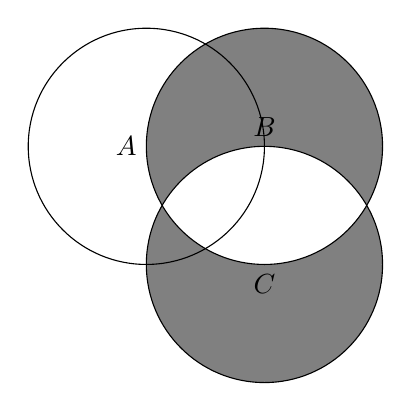
\begin{tikzpicture}
          % Define circles for A, B, and C
          \def\circleA{(0,0) circle (1.5cm)}
          \def\circleB{(1.5,0) circle (1.5cm)}
          \def\circleC{(1.5,-1.5) circle (1.5cm)}
        
          % Fill A
          \begin{scope}
            \fill[white] \circleA;
          \end{scope}
        
          % Fill B
          \begin{scope}
            \clip \circleB;
            \fill[gray] \circleB;
            \clip \circleC;
            \fill[white] \circleC;
          \end{scope}

          %Fill C
          \begin{scope}
              \clip \circleC;
              \fill[gray] \circleC;
              \clip \circleB;
              \fill[white] \circleB;
          \end{scope}
          
          % Outline the circles and label them
          \draw \circleA node [text=black, left] {$A$};
          \draw \circleB node [text=black, above] {$B$};
          \draw \circleC node [text=black, below] {$C$};
        \end{tikzpicture}

        \

    Hence, $A \mybackslash (B \triangle C)$ looks like:
    
    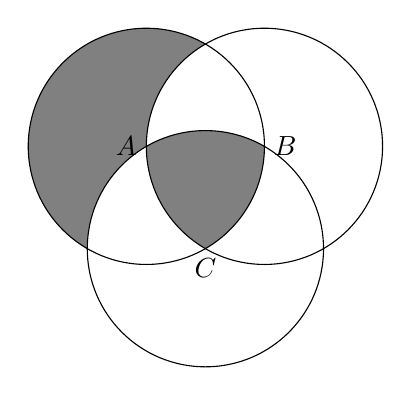
\begin{tikzpicture}
      % Define circles for A, B, and C
      \def\circleA{(0,0) circle (1.5cm)}
      \def\circleB{(1.5,0) circle (1.5cm)}
      \def\circleC{(0.75,-1.3) circle (1.5cm)}
    
      % Shade for A excluding (B \ C) and (C \ B)
      \begin{scope}
        \clip \circleA;
        \fill[gray] \circleA;
        \clip \circleB;
        \fill[white] \circleB;
      \end{scope}
      
      \begin{scope}
        \clip \circleA;
        \clip \circleC;
        \fill[white] \circleC;
      \end{scope}
    
      % Shade the intersection of A, B, and C with a different color
      \begin{scope}
        \clip \circleA;
        \clip \circleB;
        \clip \circleC;
        \fill[gray] \circleC;
      \end{scope}
      
      % Outline the circles and label them
      \draw \circleA node [text=black, left] {$A$};
      \draw \circleB node [text=black, right] {$B$};
      \draw \circleC node [text=black, below] {$C$};
    \end{tikzpicture}

    \pagebreak
    
    Meanwhile, $(B \triangle C) \mybackslash A$ looks like as shown below:

    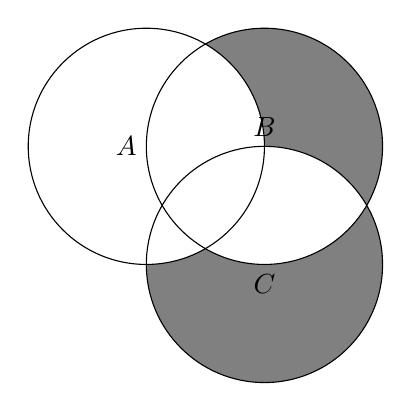
\begin{tikzpicture}
      % Define circles for A, B, and C
      \def\circleA{(0,0) circle (1.5cm)}
      \def\circleB{(1.5,0) circle (1.5cm)}
      \def\circleC{(1.5,-1.5) circle (1.5cm)}
    
      % Fill the symmetric difference of B and C
      \begin{scope}
        \clip \circleB \circleC; % Start with B and C
        \fill[gray] \circleB \circleC; % Fill B and C
        \clip \circleA; % Remove parts that overlap with A
        \fill[white] \circleA;
      \end{scope}
    
      \begin{scope}
        \clip \circleB;
        \clip \circleC;
        \fill[white] \circleC;
      \end{scope}
    
      \begin{scope}
        \clip \circleC;
        \clip \circleB;
        \fill[white] \circleB;
      \end{scope}
    
      % Outline the circles and label them
      \draw \circleA node [text=black, left] {$A$};
      \draw \circleB node [text=black, above] {$B$};
      \draw \circleC node [text=black, below] {$C$};
    \end{tikzpicture}

    Finally, we consider the union, i.e., $A \triangle (B \triangle C) \equiv (A \mybackslash (B \triangle C)) \cup ((B \triangle C) \mybackslash A)$ to get:
    
    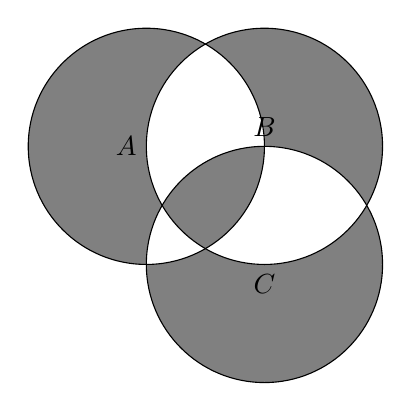
\begin{tikzpicture}
      % Define circles for A, B, and C
      \def\circleA{(0,0) circle (1.5cm)}
      \def\circleB{(1.5,0) circle (1.5cm)}
      \def\circleC{(1.5,-1.5) circle (1.5cm)}

      % Shade for A excluding (B \ C) and (C \ B)
      \begin{scope}
        \clip \circleA;
        \fill[gray] \circleA;
        \clip \circleB;
        \fill[white] \circleB;
      \end{scope}
      
      % Fill the symmetric difference of B and C
      \begin{scope}
        \clip \circleB \circleC; % Start with B and C
        \fill[gray] \circleB \circleC; % Fill B and C
        \clip \circleA; % Remove parts that overlap with A
        \fill[white] \circleA;
      \end{scope}
    
      \begin{scope}
        \clip \circleB;
        \clip \circleC;
        \fill[white] \circleC;
      \end{scope}
    
      \begin{scope}
        \clip \circleC;
        \clip \circleB;
        \fill[white] \circleB;
      \end{scope}

      % Shade the intersection of A, B, and C with a different color
      \begin{scope}
        \clip \circleA;
        \clip \circleB;
        \clip \circleC;
        \fill[gray] \circleC;
      \end{scope}
      
      % Outline the circles and label them
      \draw \circleA node [text=black, left] {$A$};
      \draw \circleB node [text=black, above] {$B$};
      \draw \circleC node [text=black, below] {$C$};
    \end{tikzpicture}
    
    \item Now, when we consider $(A \triangle B) \triangle C \equiv ((A \triangle B) \mybackslash C) \cup (C \mybackslash (A \triangle B))$, we first draw the LHS of the union below, i.e., $(A \triangle B) \mybackslash C$.

    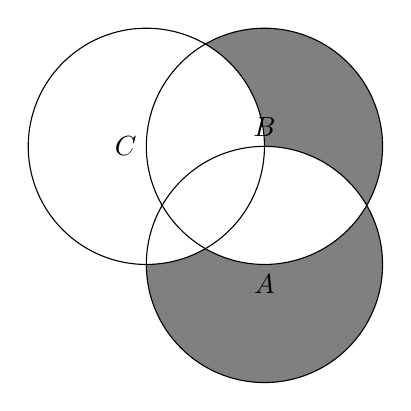
\begin{tikzpicture}
      % Define circles for A, B, and C
      \def\circleA{(0,0) circle (1.5cm)}
      \def\circleB{(1.5,0) circle (1.5cm)}
      \def\circleC{(1.5,-1.5) circle (1.5cm)}
    
      % Fill the symmetric difference of B and C
      \begin{scope}
        \clip \circleB \circleC; % Start with B and C
        \fill[gray] \circleB \circleC; % Fill B and C
        \clip \circleA; % Remove parts that overlap with A
        \fill[white] \circleA;
      \end{scope}
    
      \begin{scope}
        \clip \circleB;
        \clip \circleC;
        \fill[white] \circleC;
      \end{scope}
    
      \begin{scope}
        \clip \circleC;
        \clip \circleB;
        \fill[white] \circleB;
      \end{scope}
    
      % Outline the circles and label them
      \draw \circleA node [text=black, left] {$C$};
      \draw \circleB node [text=black, above] {$B$};
      \draw \circleC node [text=black, below] {$A$};
    \end{tikzpicture}

    \pagebreak
    Meanwhile $C \mybackslash (A \triangle B)$ looks like:

    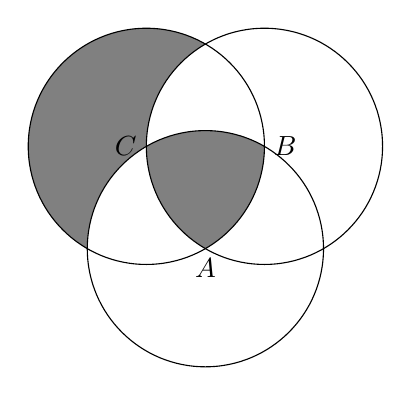
\begin{tikzpicture}
      % Define circles for A, B, and C
      \def\circleA{(0,0) circle (1.5cm)}
      \def\circleB{(1.5,0) circle (1.5cm)}
      \def\circleC{(0.75,-1.3) circle (1.5cm)}
    
      % Shade for A excluding (B \ C) and (C \ B)
      \begin{scope}
        \clip \circleA;
        \fill[gray] \circleA;
        \clip \circleB;
        \fill[white] \circleB;
      \end{scope}
      
      \begin{scope}
        \clip \circleA;
        \clip \circleC;
        \fill[white] \circleC;
      \end{scope}
    
      % Shade the intersection of A, B, and C with a different color
      \begin{scope}
        \clip \circleA;
        \clip \circleB;
        \clip \circleC;
        \fill[gray] \circleC;
      \end{scope}
      
      % Outline the circles and label them
      \draw \circleA node [text=black, left] {$C$};
      \draw \circleB node [text=black, right] {$B$};
      \draw \circleC node [text=black, below] {$A$};
    \end{tikzpicture}

    Finally, we consider the union, i.e., $(A \triangle B) \triangle C \equiv ((A \triangle B) \mybackslash C) \cup (C \mybackslash (A \triangle B))$ to get:
    
    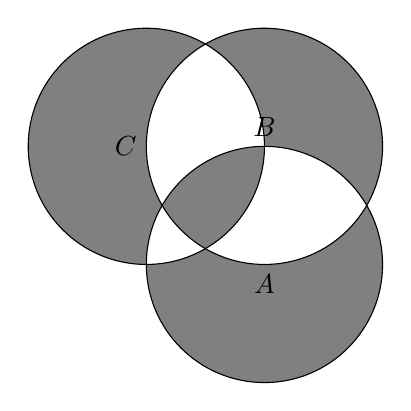
\begin{tikzpicture}
      % Define circles for A, B, and C
      \def\circleA{(0,0) circle (1.5cm)}
      \def\circleB{(1.5,0) circle (1.5cm)}
      \def\circleC{(1.5,-1.5) circle (1.5cm)}

      % Shade for A excluding (B \ C) and (C \ B)
      \begin{scope}
        \clip \circleA;
        \fill[gray] \circleA;
        \clip \circleB;
        \fill[white] \circleB;
      \end{scope}
      
      % Fill the symmetric difference of B and C
      \begin{scope}
        \clip \circleB \circleC; % Start with B and C
        \fill[gray] \circleB \circleC; % Fill B and C
        \clip \circleA; % Remove parts that overlap with A
        \fill[white] \circleA;
      \end{scope}
    
      \begin{scope}
        \clip \circleB;
        \clip \circleC;
        \fill[white] \circleC;
      \end{scope}
    
      \begin{scope}
        \clip \circleC;
        \clip \circleB;
        \fill[white] \circleB;
      \end{scope}

      % Shade the intersection of A, B, and C with a different color
      \begin{scope}
        \clip \circleA;
        \clip \circleB;
        \clip \circleC;
        \fill[gray] \circleC;
      \end{scope}
      
      % Outline the circles and label them
      \draw \circleA node [text=black, left] {$C$};
      \draw \circleB node [text=black, above] {$B$};
      \draw \circleC node [text=black, below] {$A$};
    \end{tikzpicture}
\end{itemize}

We note that we get the same diagram in both cases. Thus proving that the associative law holds.
\pagebreak

\section*{Exercise 13}
\addcontentsline{toc}{section}{Exercise 13}
Use any method you wish to verify the following identities:

\begin{enumerate}[label=(\alph*)]
\item $(A \triangle B) \cup C = (A \cup C) \triangle (B \mybackslash C)$.
\item $(A \triangle B) \cap C = (A \cap C) \triangle (B \cap C)$.
\item $(A \triangle B) \mybackslash C = (A \mybackslash C) \triangle (B \mybackslash C)$.
\end{enumerate}

\textbf{Solution:} \\
\textbf{13(a)} Below we prove that $(A \triangle B) \cup C = (A \cup C) \triangle (B \mybackslash C)$.
\begin{alignat*}{2}
&x \in (A \cup C) \triangle (B \mybackslash C) && \quad \textbf{(1)} \\
&\equiv x \in [(A \cup C) \cup (B \mybackslash C)] \mybackslash [(A \cup C) \cap (B \mybackslash C)] && \quad \textbf{(2)}\\
&\equiv [x \in (A \cup C) \cup (B \mybackslash C)] \wedge \neg [x \in (A \cup C) \cap (B \mybackslash C)] && \quad \textbf{(3)}\\
&\equiv {[(x \in A \vee x \in C) \vee (x \in B \wedge \neg (x \in C))]} \wedge \neg [(x \in A \vee x \in C) \wedge (x \in B \wedge \neg (x \in C))] && \quad \textbf{(4)}\\
&\equiv {[(x \in A \vee x \in C) \vee x \in B] \wedge [(x \in A \vee x \in C) \vee \neg (x \in C)]} \wedge \neg [(x \in A \vee x \in C) \wedge (x \in B \wedge \neg (x \in C))] && \quad \textbf{(5)}\\
&\equiv {[(x \in A \vee x \in B) \vee x \in C] \wedge (x \in A \vee x \in C \vee \neg (x \in C))} \wedge \neg [(x \in A \vee x \in C) \wedge (x \in B \wedge \neg (x \in C))] && \quad \textbf{(6)}\\
&\equiv [x \in Q \wedge (x \in A \vee x \in C \vee \neg (x \in C))] \wedge \neg [(x \in A \vee x \in C) \wedge (x \in B \wedge \neg (x \in C))] && \quad \textbf{(7)}\\
&\equiv [x \in Q \wedge \text{Tautology}] \wedge \neg [(x \in A \vee x \in C) \wedge (x \in B \wedge \neg (x \in C))] && \quad \textbf{(8)}\\
&\equiv [x \in Q \wedge \text{Tautology}] \wedge {\neg [x \in A \vee x \in C] \vee \neg [x \in B \wedge \neg (x \in C)]} && \quad \textbf{(9)}\\
&\equiv [x \in Q \wedge \text{Tautology}] \wedge {[\neg (x \in A) \wedge \neg (x \in C)] \vee [\neg (x \in B) \vee x \in C]} && \quad \textbf{(10)}\\
&\equiv [x \in Q \wedge \text{Tautology}] \wedge {[(\neg (x \in A) \wedge \neg (x \in C)) \vee \neg (x \in B)] \vee [(\neg (x \in A) \wedge \neg (x \in C)) \vee x \in C]} && \quad \textbf{(11)}\\
&\equiv [x \in Q \wedge \text{Tautology}] \wedge {[(\neg (x \in A) \vee \neg (x \in B)) \wedge (\neg (x \in C) \vee \neg (x \in B))] \vee [(\neg (x \in A) \wedge \neg (x \in C)) \vee x \in C]} && \quad \textbf{(12)}\\
&\equiv [x \in Q \wedge \text{Tautology}] \wedge {[x \in P \wedge (\neg (x \in C) \vee \neg (x \in B))] \vee [(\neg (x \in A) \wedge \neg (x \in C)) \vee x \in C]} && \quad \textbf{(13)}\\
&\equiv [x \in Q \wedge \text{Tautology}] \wedge {[x \in P \wedge (\neg (x \in C) \vee \neg (x \in B))] \vee [(\neg (x \in A) \vee x \in C) \wedge (x \in C \vee \neg (x \in C))]} && \quad \textbf{(14)}\\
&\equiv [x \in Q \wedge \text{Tautology}] \wedge {[x \in P \wedge (\neg (x \in C) \vee \neg (x \in B))] \vee [(\neg (x \in A) \vee x \in C) \wedge \text{Tautology}]} && \quad \textbf{(15)}\\
&\equiv (x \in Q) \wedge {[x \in P \wedge (\neg (x \in C) \vee \neg (x \in B))] \vee [\neg (x \in A) \vee x \in C]} && \quad \textbf{(16)}\\
&\equiv (x \in Q) \wedge {[x \in P \wedge \neg (x \in C)] \vee [P \wedge \neg (x \in B)] \vee [\neg (x \in A) \vee x \in C]} && \quad \textbf{(17)}\\
&\equiv (x \in Q) \wedge [(x \in P \wedge \neg (x \in C)) \vee \neg (x \in A) \vee [P \wedge \neg (x \in B)] \vee x \in C] && \quad \textbf{(18)}\\
&\equiv (x \in Q) \wedge [(x \in P \wedge \neg (x \in C)) \vee \neg (x \in A) \vee [(\neg (x \in A) \vee \neg (x \in B)) \wedge \neg (x \in B)] \vee x \in C] && \quad \textbf{(19)}\\
&\equiv (x \in Q) \wedge [(x \in P \wedge \neg (x \in C)) \vee \neg (x \in A) \vee \neg (x \in B) \vee x \in C] && \quad \textbf{(20)}\\
&\equiv (x \in Q) \wedge [(x \in P \wedge \neg (x \in C)) \vee x \in P \vee x \in C] && \quad \textbf{(21)}\\
&\equiv (x \in Q) \wedge [((x \in P \wedge \neg (x \in C)) \vee x \in P) \vee x \in C] && \quad \textbf{(22)}\\
&\equiv (x \in Q) \wedge [(x \in P \vee (x \in P \wedge \neg (x \in C))) \vee x \in C] && \quad \textbf{(23)}\\
&\equiv (x \in Q) \wedge [x \in P \vee x \in C] && \quad \textbf{(24)}\\
&\equiv (x \in Q) \wedge [(\neg (x \in A) \vee \neg (x \in B)) \vee x \in C] && \quad \textbf{(25)}\\
&\equiv [(x \in A \vee x \in B) \vee x \in C] \wedge [(\neg (x \in A) \vee \neg (x \in B)) \vee x \in C] && \quad \textbf{(26)}\\
&\equiv [(x \in A \vee x \in B) \wedge (\neg (x \in A) \vee \neg (x \in B))] \vee (x \in C) && \quad \textbf{(27)}\\
&\equiv [(x \in A \vee x \in B) \wedge \neg (x \in A \wedge x \in B)] \vee (x \in C) && \quad \textbf{(28)}\\
&\equiv [(x \in A \cup B) \wedge \neg (x \in A \cap B)] \vee (x \in C) && \quad \textbf{(29)}\\
&\equiv [x \in (A \cup B) \mybackslash (A \cap B)] \vee (x \in C) && \quad \textbf{(30)}\\
&\equiv (x \in A \triangle B) \vee (x \in C) && \quad \textbf{(31)}\\
&\equiv x \in (A \triangle B) \cup C && \quad \textbf{(32)}\\
&\qed
\end{alignat*}

Below is the corresponding chain of justification of the \textbf{13(a)} proof.
\begin{alignat*}{2}
&\textbf{(1)} && \quad \text{RHS}\\
&\textbf{(2)} && \quad \text{Def. of Symmetric Difference}\\
&\textbf{(3)} && \quad \text{Def. of Difference of Sets}\\
&\textbf{(4)} && \quad \text{Def. of Union, Intersection and Difference of Sets}\\
&\textbf{(5)} && \quad \text{Distributive Law}\\
&\textbf{(6)} && \quad \text{Associative and Commutative Law}\\
&\textbf{(7)} && \quad \text{Substitution where $x \in Q \equiv (x \in A \vee x \in B) \vee x \in C$}\\
&\textbf{(8)} && \quad \text{Definition of Tautology}\\
&\textbf{(9)} && \quad \text{DeMorgan's Law}\\
&\textbf{(10)} && \quad \text{DeMorgan's Law}\\
&\textbf{(11)} && \quad \text{Distributive Law}\\
&\textbf{(12)} && \quad \text{Distributive Law}\\
&\textbf{(13)} && \quad \text{Substitution where $x \in P \equiv \neg (x \in A) \vee \neg (x \in B)$}\\
&\textbf{(14)} && \quad \text{Definition of Tautology}\\
&\textbf{(15)} && \quad \text{Tautology Law}\\
&\textbf{(16)} && \quad \text{Commutative Law and Associative Law}\\
&\textbf{(17)} && \quad \text{Distributive Law}\\
&\textbf{(18)} && \quad \text{Commutative Law}\\
&\textbf{(19)} && \quad \text{Substitution where $x \in P \equiv \neg (x \in A) \vee \neg (x \in B)$}\\
&\textbf{(20)} && \quad \text{Absorption Law $(\neg (x \in B) \equiv (\neg (x \in A) \vee \neg (x \in B)) \wedge \neg (x \in B))$}\\
&\textbf{(21)} && \quad \text{Substitution where $x \in P \equiv \neg (x \in A) \vee \neg (x \in B)$}\\
&\textbf{(22)} && \quad \text{Associative Law}\\
&\textbf{(23)} && \quad \text{Commutative Law}\\
&\textbf{(24)} && \quad \text{Absorption Law $(P \equiv P \vee (P \wedge \neg C))$}\\
&\textbf{(25)} && \quad \text{Substitution where $x \in P \equiv \neg (x \in A) \vee \neg (x \in B)$}\\
&\textbf{(26)} && \quad \text{Substitution where $x \in Q \equiv (x \in A \vee x \in B) \vee x \in C$}\\
&\textbf{(27)} && \quad \text{Distributive Law}\\
&\textbf{(28)} && \quad \text{DeMorgan's Law}\\
&\textbf{(29)} && \quad \text{Def. of Union and Intersection of Sets}\\
&\textbf{(30)} && \quad \text{Def. of Difference of Sets}\\
&\textbf{(31)} && \quad \text{Def. of Symmetric Difference}\\
&\textbf{(32)} && \quad \text{Def. of Union of Sets, LHS}\\        
\end{alignat*}
\pagebreak

\textbf{13(b)} Below we prove that $(A \triangle B) \cap C = (A \cap C) \triangle (B \cap C)$.
\begin{alignat*}{2}
&x \in (A \cap C) \triangle (B \cap C) && \quad \textbf{(1)}\\
&\equiv x \in [(A \cap C) \cup (B \cap C)] \setminus [(A \cap C) \cap (B \cap C)] && \quad \textbf{(2)}\\
&\equiv [x \in (A \cap C) \cup (B \cap C)] \wedge \neg [x \in (A \cap C) \cap (B \cap C)] && \quad \textbf{(3)}\\
&\equiv \{[x \in A \wedge x \in C] \vee [x \in B \wedge x \in C]\} \wedge \neg \{[x \in A \wedge x \in C] \wedge [x \in B \wedge x \in C]\} && \quad \textbf{(4)}\\
&\equiv \{(x \in A \vee x \in B) \wedge x \in C\} \wedge \neg \{[x \in A \wedge x \in C] \wedge [x \in B \wedge x \in C]\} && \quad \textbf{(5)}\\
&\equiv [(x \in A \vee x \in B) \wedge x \in C] \wedge \neg [x \in A \wedge x \in C \wedge x \in B \wedge x \in C] && \quad \textbf{(6)}\\
&\equiv [(x \in A \vee x \in B) \wedge x \in C] \wedge \neg [x \in A \wedge x \in B \wedge (x \in C \wedge x \in C)] && \quad \textbf{(7)}\\
&\equiv [(x \in A \vee x \in B) \wedge x \in C] \wedge \neg [x \in A \wedge x \in B \wedge x \in C] && \quad \textbf{(8)}\\
&\equiv [(x \in A \vee x \in B) \wedge x \in C] \wedge [\neg (x \in A \wedge x \in B) \vee \neg (x \in C)] && \quad \textbf{(9)}\\
&\equiv \{[(x \in A \vee x \in B) \wedge x \in C] \wedge \neg (x \in A \wedge x \in B)\} \vee \{[(x \in A \vee x \in B) \wedge x \in C] \wedge \neg (x \in C)\} && \quad \textbf{(10)}\\
&\equiv \{[(x \in A \vee x \in B) \wedge x \in C] \wedge \neg (x \in A \wedge x \in B)\} \vee \{(x \in A \vee x \in B) \wedge [x \in C \wedge \neg (x \in C)]\} && \quad \textbf{(11)}\\
&\equiv \{[(x \in A \vee x \in B) \wedge x \in C] \wedge \neg (x \in A \wedge x \in B)\} \vee \{(x \in A \vee x \in B) \wedge \text{Contradiction}\} && \quad \textbf{(12)}\\
&\equiv \{[(x \in A \vee x \in B) \wedge x \in C] \wedge \neg (x \in A \wedge x \in B)\} \vee (\text{Contradiction}) && \quad \textbf{(13)}\\
&\equiv \{[(x \in A \vee x \in B) \wedge x \in C] \wedge \neg (x \in A \wedge x \in B)\} && \quad \textbf{(14)}\\
&\equiv (x \in A \vee x \in B) \wedge (x \in C) \wedge \neg (x \in A \wedge x \in B) && \quad \textbf{(15)}\\
&\equiv (x \in A \vee x \in B) \wedge \neg (x \in A \wedge x \in B) \wedge (x \in C)  && \quad \textbf{(16)}\\
&\equiv (x \in A \cup B) \wedge \neg (x \in A \cap B) \wedge (x \in C)  && \quad \textbf{(17)}\\
&\equiv [(x \in A \cup B) \wedge \neg (x \in A \cap B)] \wedge (x \in C)  && \quad \textbf{(18)}\\
&\equiv (x \in A \triangle B) \wedge (x \in C)  && \quad \textbf{(19)}\\
&\equiv x \in (A \triangle B) \cap C  && \quad \textbf{(20)}\\
&\qed \\
\end{alignat*}

\pagebreak

Below is the corresponding chain of justification of the \textbf{13(b)} proof.
\begin{alignat*}{2}
&\textbf{(1)} && \quad \text{RHS}\\
&\textbf{(2)} && \quad \text{Def. of Symmetric Difference}\\
&\textbf{(3)} && \quad \text{Def. of Difference of Sets}\\
&\textbf{(4)} && \quad \text{Def. of Union and Intersection of Sets}\\
&\textbf{(5)} && \quad \text{Distributive Law}\\
&\textbf{(6)} && \quad \text{Associative Law}\\
&\textbf{(7)} && \quad \text{Associative Law and Commutative Law}\\
&\textbf{(8)} && \quad \text{Idempotent Law}\\
&\textbf{(9)} && \quad \text{DeMorgan's Law}\\
&\textbf{(10)} && \quad \text{Distributive Law}\\
&\textbf{(11)} && \quad \text{Associative Law}\\
&\textbf{(12)} && \quad \text{Def. of Contradiction}\\
&\textbf{(13)} && \quad \text{Contradiction Law}\\
&\textbf{(14)} && \quad \text{Contradiction Law}\\
&\textbf{(15)} && \quad \text{Associative Law}\\
&\textbf{(16)} && \quad \text{Commutative Law}\\
&\textbf{(17)} && \quad \text{Def. of Union and Intersection of Sets}\\
&\textbf{(18)} && \quad \text{Associative Law}\\
&\textbf{(19)} && \quad \text{Def. of Symmetric Difference}\\
&\textbf{(20)} && \quad \text{Def. of Intersection of Sets, LHS}\\
\end{alignat*}
\pagebreak

\textbf{13(c)} Below we prove that $(A \triangle B) \mybackslash C = (A \mybackslash C) \triangle (B \mybackslash C)$.
\begin{alignat*}{2}
& x \in (A \mybackslash C) \triangle (B \mybackslash C) && \quad \textbf{(1)}\\
&\equiv x \in [(A \setminus C) \cup (B \setminus C)] \setminus [(A \setminus C) \cap (B \setminus C)] && \quad \textbf{(2)}\\
&\equiv [x \in (A \setminus C) \cup (B \setminus C)] \wedge \neg [x \in (A \setminus C) \cap (B \setminus C)] && \quad \textbf{(3)}\\
&\equiv [(x \in A \setminus C) \vee  (x \in B \setminus C)] \wedge \neg [(x \in A \setminus C) \wedge (x \in B \setminus C)] && \quad \textbf{(4)}\\
&\equiv \{[x \in A \wedge \neg (x \in C)] \vee  [x \in B \wedge \neg (x \in C)]\} \wedge \neg \{(x \in A \setminus C) \wedge (x \in B \setminus C)\} && \quad \textbf{(5)}\\
&\equiv [(x \in A \vee x \in B) \wedge \neg (x \in C)] \wedge \neg \{(x \in A \setminus C) \wedge (x \in B \setminus C)\} && \quad \textbf{(6)}\\
&\equiv [(x \in A \vee x \in B) \wedge \neg (x \in C)] \wedge \neg \{[x \in A \wedge \neg (x \in C)] \wedge [x \in B \wedge \neg (x \in C)]\} && \quad \textbf{(7)}\\
&\equiv [(x \in A \vee x \in B) \wedge \neg (x \in C)] \wedge \neg [x \in A \wedge \neg (x \in C) \wedge x \in B \wedge \neg (x \in C)] && \quad \textbf{(8)}\\
&\equiv [(x \in A \vee x \in B) \wedge \neg (x \in C)] \wedge \neg [x \in A \wedge x \in B \wedge [\neg (x \in C) \wedge \neg (x \in C)]] && \quad \textbf{(9)}\\
&\equiv [(x \in A \vee x \in B) \wedge \neg (x \in C)] \wedge \neg [x \in A \wedge x \in B \wedge \neg (x \in C)] && \quad \textbf{(10)}\\
&\equiv [(x \in A \vee x \in B) \wedge \neg (x \in C)] \wedge [\neg (x \in A \wedge x \in B) \vee x \in C] && \quad \textbf{(11)}\\
&\equiv \{[(x \in A \vee x \in B) \wedge \neg (x \in C)] \wedge \neg (x \in A \wedge x \in B)\} \vee \{[(x \in A \vee x \in B) \wedge \neg (x \in C)] \wedge x \in C\} && \quad \textbf{(12)}\\
&\equiv \{[(x \in A \vee x \in B) \wedge \neg (x \in C)] \wedge \neg (x \in A \wedge x \in B)\} \vee \{(x \in A \vee x \in B) \wedge [\neg (x \in C) \wedge x \in C]\} && \quad \textbf{(13)}\\
&\equiv \{[(x \in A \vee x \in B) \wedge \neg (x \in C)] \wedge \neg (x \in A \wedge x \in B)\} \vee [(x \in A \vee x \in B) \wedge \text{Contradiction}] && \quad \textbf{(14)}\\
&\equiv \{[(x \in A \vee x \in B) \wedge \neg (x \in C)] \wedge \neg (x \in A \wedge x \in B)\} \vee \text{Contradiction} && \quad \textbf{(15)}\\
&\equiv [(x \in A \vee x \in B) \wedge \neg (x \in C)] \wedge \neg (x \in A \wedge x \in B) && \quad \textbf{(16)}\\
&\equiv (x \in A \vee x \in B) \wedge \neg (x \in C) \wedge \neg (x \in A \wedge x \in B) && \quad \textbf{(17)}\\
&\equiv (x \in A \vee x \in B) \wedge \neg (x \in A \wedge x \in B) \wedge \neg (x \in C) && \quad \textbf{(18)}\\
&\equiv [(x \in A \vee x \in B) \wedge \neg (x \in A \wedge x \in B)] \wedge \neg (x \in C) && \quad \textbf{(19)}\\
&\equiv [(x \in A \cup B) \wedge \neg (x \in A \cap B)] \wedge \neg (x \in C) && \quad \textbf{(20)}\\
&\equiv [x \in (A \cup B) \setminus (A \cap B)] \wedge \neg (x \in C) && \quad \textbf{(21)}\\
&\equiv x \in (A \triangle B) \wedge \neg (x \in C) && \quad \textbf{(22)}\\
&\equiv x \in (A \triangle B) \setminus C && \quad \textbf{(23)}\\
&\qed
\end{alignat*}
\pagebreak

Below is the corresponding chain of justification of the \textbf{13(c)} proof.
\begin{alignat*}{2}
&\textbf{(1)} && \quad \text{RHS}\\
&\textbf{(2)} && \quad \text{Def. of Symmetric Difference}\\
&\textbf{(3)} && \quad \text{Def. of Difference  of Sets}\\
&\textbf{(4)} && \quad \text{Def. of Union and Intersection of Sets}\\
&\textbf{(5)} && \quad \text{Def. of Difference  of Sets}\\
&\textbf{(6)} && \quad \text{Distributive Law}\\
&\textbf{(7)} && \quad \text{Def. of Difference  of Sets}\\
&\textbf{(8)} && \quad \text{Associative Law}\\
&\textbf{(9)} && \quad \text{Associative and Commutative Law}\\
&\textbf{(10)} && \quad \text{Idempotent Law}\\
&\textbf{(11)} && \quad \text{DeMorgan's Law}\\
&\textbf{(12)} && \quad \text{Distributive Law}\\
&\textbf{(15)} && \quad \text{Contradiction Law}\\
&\textbf{(14)} && \quad \text{Def. of Contradiction}\\
&\textbf{(15)} && \quad \text{Contradiction Law}\\
&\textbf{(16)} && \quad \text{Contradiction Law}\\
&\textbf{(17)} && \quad \text{Associative Law}\\
&\textbf{(18)} && \quad \text{Commutative Law}\\
&\textbf{(19)} && \quad \text{Associative Law}\\
&\textbf{(20)} && \quad \text{Def. of Union and Intersection of Sets}\\
&\textbf{(21)} && \quad \text{Def. of Difference of Sets}\\
&\textbf{(22)} && \quad \text{Def. of Symmetric Difference}\\
&\textbf{(23)} && \quad \text{Def. of Difference of Sets, LHS}\\
\end{alignat*}
\pagebreak

\section*{Exercise 14}
\addcontentsline{toc}{section}{Exercise 14}
Note that the associative laws say only that the parentheses are unnecessary when combining \textit{three} statements with $\wedge$ or $\vee$. In fact, these laws can be used to justify leaving parentheses out when more than three statements are combined. Use associative laws to show that $[P \wedge (Q \wedge R)] \wedge S$ is equivalent $(P \wedge Q) \wedge (R \wedge S)$.

\textbf{Solution:}
\begin{alignat*}{2}
    [P \wedge (Q \wedge R)] \wedge S & \equiv [P \wedge Q \wedge R] \wedge S \quad && \text{(Associative Law)} \\
    & \equiv [(P \wedge Q) \wedge R] \wedge S \quad && \text{(Associative Law)} \\
    & \equiv (A \wedge R) \wedge S \quad && \text{(Let $A \equiv P \wedge Q$)} \\
    & \equiv A \wedge R \wedge S \quad && \text{(Associative Law)} \\
    & \equiv A \wedge (R \wedge S) \quad && \text{(Associative Law)} \\
    & \equiv (P \wedge Q) \wedge (R \wedge S) \quad && \text{(Since $A \equiv P \wedge Q$)} \\
\end{alignat*}

\pagebreak

\section*{Exercise 15}
\addcontentsline{toc}{section}{Exercise 15}
Fill in the blanks to make true identities:
\begin{enumerate}[label=(\alph*)]
\item $(A \triangle B) \cap C = (C \setminus A) \triangle $ \makebox[1cm]{\hrulefill}.
\item $C \setminus (A \triangle B) = (A \cap C) \triangle $ \makebox[1cm]{\hrulefill}.
\item $(B \setminus A) \triangle C = (A \triangle C) \triangle $ \makebox[1cm]{\hrulefill}.
\end{enumerate}

\textbf{Solution:} 
\

\textbf{15(a)}: Consider that $(A \triangle B) \cap C = [(A \wedge C) \vee (B \wedge C)] \wedge \neg (A \wedge B)$. \\ The corresponding Venn diagram is shown below. \\
Note the symmetry, we guess that $(A \triangle B) \cap C = (C \setminus A) \triangle (C \setminus B)$.

\

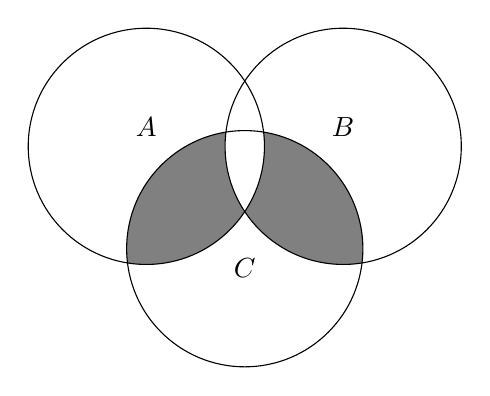
\begin{tikzpicture}
% Define circles for A, B, and C
\def\circleA{(-0.5,0) circle (1.5cm)}
\def\circleB{(2,0) circle (1.5cm)}
\def\circleC{(0.75,-1.3) circle (1.5cm)}

% Shade (A and C) excluding (A and B)
\begin{scope}
\clip \circleA;
\clip \circleC;
\fill[gray] \circleC;
\clip \circleB;
\fill[white] \circleB;
\end{scope}

% Shade (B and C) excluding (A and B)
\begin{scope}
\clip \circleB;
\clip \circleC;
\fill[gray] \circleC;
\clip \circleA;
\fill[white] \circleA;
\end{scope}

% Outline the circles and label them
\draw \circleA node [text=black, above] {$A$};
\draw \circleB node [text=black, above] {$B$};
\draw \circleC node [text=black, below] {$C$};
\end{tikzpicture}
\pagebreak

Below is the prove for \textbf{15(a)}. 
\begin{alignat*}{2}
&x \in (C \setminus A) \triangle (C \setminus B) && \quad \textbf{(1)}\\
&\equiv x \in [(C \setminus A) \cup (C \setminus B)] \setminus [(C \setminus A) \cap (C \setminus B)] && \quad \textbf{(2)}\\
&\equiv x \in [(C \setminus A) \cup (C \setminus B)] \setminus Q && \quad \textbf{(3)}\\
&\equiv [x \in (C \setminus A) \cup (C \setminus B)] \wedge \neg (x \in Q) && \quad \textbf{(4)}\\
&\equiv [x \in C \setminus A \vee x \in C \setminus B] \wedge \neg (x \in Q) && \quad \textbf{(5)}\\
&\equiv \{[x \in C \wedge \neg (x \in A)] \vee [x \in C \wedge \neg (x \in B)]\} \wedge \neg (x \in Q) && \quad \textbf{(6)}\\
&\equiv \{([x \in C \wedge \neg (x \in A)] \vee x \in C) \wedge ([x \in C \wedge \neg (x \in A)] \vee \neg [x \in B])\} \wedge \neg (x \in Q) && \quad \textbf{(7)}\\
&\equiv \{(x \in C) \wedge ([x \in C \wedge \neg (x \in A)] \vee \neg [x \in B])\} \wedge \neg (x \in Q) && \quad \textbf{(8)}\\
&\equiv \{(x \in C \wedge [x \in C \wedge \neg (x \in A)]) \vee [x \in C \wedge \neg (x \in B)]\} \wedge \neg (x \in Q) && \quad \textbf{(9)}\\
&\equiv \{([x \in C \wedge x \in C] \wedge \neg (x \in A)) \vee [x \in C \wedge \neg (x \in B)]\} \wedge \neg (x \in Q) && \quad \textbf{(10)}\\
&\equiv \{[x \in C \wedge \neg (x \in A)] \vee [x \in C \wedge \neg (x \in B)]\} \wedge \neg (x \in Q) && \quad \textbf{(11)}\\
&\equiv \{x \in C \wedge [\neg (x \in A) \vee \neg (x \in B)]\} \wedge \neg (x \in Q) && \quad \textbf{(12)}\\
&\equiv \{x \in C \wedge \neg [x \in A \wedge x \in B]\} \wedge \neg (x \in Q) && \quad \textbf{(13)}\\
&\equiv \{x \in C \wedge \neg [x \in A \wedge x \in B]\} \wedge \neg \{x \in [(C \setminus A) \cap (C \setminus B)]\} && \quad \textbf{(14)}\\
&\equiv \{x \in C \wedge \neg [x \in A \wedge x \in B]\} \wedge \neg \{[x \in C \wedge \neg (x \in A)] \wedge [x \in C \wedge \neg (x \in B)]\} && \quad \textbf{(15)}\\
&\equiv \{x \in C \wedge \neg [x \in A \wedge x \in B]\} \wedge \neg \{x \in C \wedge \neg (x \in A) \wedge x \in C \wedge \neg (x \in B)\} && \quad \textbf{(16)}\\
&\equiv \{x \in C \wedge \neg [x \in A \wedge x \in B]\} \wedge \neg \{(x \in C \wedge x \in C) \wedge \neg (x \in A) \wedge \neg (x \in B)\} && \quad \textbf{(17)}\\
&\equiv \{x \in C \wedge \neg [x \in A \wedge x \in B]\} \wedge \neg \{x \in C \wedge \neg (x \in A) \wedge \neg (x \in B)\} && \quad \textbf{(18)}\\
&\equiv \{x \in C \wedge \neg [x \in A \wedge x \in B]\} \wedge \neg \{x \in C \wedge \neg [x \in A \vee x \in B]\} && \quad \textbf{(19)}\\
&\equiv \{x \in C \wedge \neg [x \in A \wedge x \in B]\} \wedge \{\neg (x \in C) \vee [x \in A \vee x \in B]\} && \quad \textbf{(20)}\\
&\equiv \{(x \in C \wedge \neg [x \in A \wedge x \in B]) \wedge \neg (x \in C)\} \vee \{(x \in C \wedge \neg [x \in A \wedge x \in B]) \wedge [x \in A \vee x \in B]\} && \quad \textbf{(21)}\\
&\equiv \{[x \in C \wedge \neg (x \in C)] \wedge \neg [x \in A \wedge x \in B]\} \vee \{x \in C \wedge \neg [x \in A \wedge x \in B] \wedge [x \in A \vee x \in B]\} && \quad \textbf{(22)}\\
&\equiv \{\text{Contradiction} \wedge \neg [x \in A \wedge x \in B]\} \vee \{x \in C \wedge \neg [x \in A \wedge x \in B] \wedge [x \in A \vee x \in B]\} && \quad \textbf{(23)}\\
&\equiv \text{Contradiction} \vee \{x \in C \wedge \neg [x \in A \wedge x \in B] \wedge [x \in A \vee x \in B]\} && \quad \textbf{(24)}\\
&\equiv x \in C \wedge \neg [x \in A \wedge x \in B] \wedge [x \in A \vee x \in B] && \quad \textbf{(25)}\\
&\equiv [(x \in A \vee x \in B) \wedge \neg (x \in A \wedge x \in B)] \wedge x \in C && \quad \textbf{(26)}\\
&\equiv [x \in A \cup B \wedge \neg (x \in A \cap B)] \wedge x \in C && \quad \textbf{(27)}\\
&\equiv [x \in (A \cup B) \setminus (A \cap B)] \wedge x \in C && \quad \textbf{(28)}\\
&\equiv [x \in A \triangle B] \wedge x \in C && \quad \textbf{(29)}\\
&\equiv x \in (A \triangle B) \cap C && \quad \textbf{(30)}\\
&\qed
\end{alignat*}
\pagebreak

Below is the chain of justification corresponding to the proof of \textbf{15(a)}.
\begin{alignat*}{2}
&\textbf{(1)} && \quad \text{RHS} \\
&\textbf{(2)} && \quad \text{Def. of Symmetric Difference} \\
&\textbf{(3)} && \quad \text{Substitution where $Q \equiv (C \setminus A) \cap (C \setminus B)$} \\
&\textbf{(4)} && \quad \text{Def. of Difference of Sets} \\
&\textbf{(5)} && \quad \text{Def. of Union of Sets} \\
&\textbf{(6)} && \quad \text{Def. of Difference of Sets} \\
&\textbf{(7)} && \quad \text{Distributive Law} \\
&\textbf{(8)} && \quad \text{Absorption Law $C \equiv C \vee (C \wedge \neg A)$} \\
&\textbf{(9)} && \quad \text{Distributive Law} \\
&\textbf{(10)} && \quad \text{Associative Law} \\
&\textbf{(11)} && \quad \text{Idempotent Law} \\
&\textbf{(12)} && \quad \text{Distributive Law} \\
&\textbf{(13)} && \quad \text{DeMorgan's Law} \\
&\textbf{(14)} && \quad \text{Substitution where $Q \equiv (C \setminus A) \cap (C \setminus B)$} \\
&\textbf{(15)} && \quad \text{Def. of Difference and Intersection of Sets} \\
&\textbf{(16)} && \quad \text{Associative Law} \\
&\textbf{(17)} && \quad \text{Associative Law and Commutative Law} \\
&\textbf{(18)} && \quad \text{Idempotent Law} \\
&\textbf{(19)} && \quad \text{DeMorgan's Law} \\
&\textbf{(20)} && \quad \text{DeMorgan's Law} \\
&\textbf{(21)} && \quad \text{Distributive Law} \\
&\textbf{(22)} && \quad \text{Associative Law and Commutative Law} \\
&\textbf{(23)} && \quad \text{Def. of Contradiction} \\
&\textbf{(24)} && \quad \text{Law of Contradiction} \\
&\textbf{(25)} && \quad \text{Law of Contradiction} \\
&\textbf{(26)} && \quad \text{Associative Law and Commutative Law} \\
&\textbf{(27)} && \quad \text{Def. of Union and Intersection of Sets} \\
&\textbf{(28)} && \quad \text{Def. of Difference of Sets} \\
&\textbf{(29)} && \quad \text{Def. of Symmetric Difference} \\
&\textbf{(30)} && \quad \text{Def. of Intersection of Sets, LHS} \\
\end{alignat*}
\pagebreak

\textbf{15(b)}: Consider that $C \setminus (A \triangle B) \equiv [A \cap B \cap C] \cup [C \cap \neg (A \cup B)]$. \\ The corresponding Venn diagram is shown below. \\
Note the symmetry, we guess that $C \setminus (A \triangle B) = (A \cap C) \triangle (B \setminus C)$.

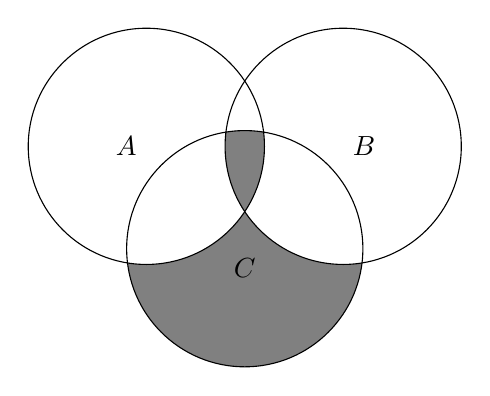
\begin{tikzpicture}
% Define circles for A, B, and C
\def\circleA{(-0.5,0) circle (1.5cm)}
\def\circleB{(2.0,0) circle (1.5cm)}
\def\circleC{(0.75,-1.3) circle (1.5cm)}

% Shade exclusively C (C not A, not B)
\begin{scope}
\clip \circleC;
\fill[gray] \circleC;
\begin{scope}
\clip \circleA;
\fill[white] \circleC;
\end{scope}
\begin{scope}
\clip \circleB;
\fill[white] \circleC;
\end{scope}
\end{scope}

% Shade the intersection of A, B, and C
\begin{scope}
\clip \circleA;
\clip \circleB;
\clip \circleC;
\fill[gray] \circleC;  % fill the intersection with the same color
\end{scope}

% Outline the circles and label them
\draw \circleA node [text=black, left] {$A$};
\draw \circleB node [text=black, right] {$B$};
\draw \circleC node [text=black, below] {$C$};
\end{tikzpicture}
\pagebreak

Below is the prove for \textbf{15(b)}.
\begin{alignat*}{2}
&x \in (A \cap C) \triangle (B \setminus C) && \quad \textbf{(1)}\\
&\equiv x \in [(A \cap C) \setminus (C \setminus B)] \cup [(C \setminus B) \setminus (A \cap C)] && \quad \textbf{(2)}\\
&\equiv x \in [(A \cap C) \setminus (C \setminus B)] \cup Q && \quad \textbf{(3)}\\
&\equiv [x \in (A \cap C) \setminus (C \setminus B)] \vee x \in Q && \quad \textbf{(4)}\\
&\equiv [(x \in A \wedge x \in C) \wedge \neg (x \in C \wedge \neg (x \in B))] \vee x \in Q && \quad \textbf{(5)}\\
&\equiv [(x \in A \wedge x \in C) \wedge (\neg (x \in C) \vee x \in B)] \vee x \in Q && \quad \textbf{(6)}\\
&\equiv \{[(x \in A \wedge x \in C) \wedge \neg (x \in C)] \vee [(x \in A \wedge x \in C) \wedge x \in B]\} \vee x \in Q && \quad \textbf{(7)}\\
&\equiv \{[x \in A \wedge (x \in C \wedge \neg (x \in C))] \vee [(x \in A \wedge x \in C) \wedge x \in B]\} \vee x \in Q && \quad \textbf{(8)}\\
&\equiv \{[x \in A \wedge \text{Contradiction}] \vee [(x \in A \wedge x \in C) \wedge x \in B]\} \vee x \in Q && \quad \textbf{(9)}\\
&\equiv \{\text{Contradiction} \vee [(x \in A \wedge x \in C) \wedge x \in B]\} \vee x \in Q && \quad \textbf{(10)}\\
&\equiv [(x \in A \wedge x \in C) \wedge x \in B] \vee x \in Q && \quad \textbf{(11)}\\
&\equiv [x \in A \wedge x \in C \wedge x \in B] \vee x \in Q && \quad \textbf{(12)}\\
&\equiv [x \in C \wedge (x \in A \wedge x \in B)] \vee x \in Q && \quad \textbf{(13)}\\
&\equiv x \in P \vee x \in Q && \quad \textbf{(14)}\\
&\equiv x \in P \vee [x \in (C \setminus B) \setminus (A \cap C)] && \quad \textbf{(15)}\\
&\equiv x \in P \vee \{(x \in C \wedge \neg (x \in B)) \wedge \neg (x \in A \wedge x \in C)\} && \quad \textbf{(16)}\\
&\equiv x \in P \vee \{(x \in C \wedge \neg ( x \in B)) \wedge (\neg (x \in A) \vee \neg (x \in C))\} && \quad \textbf{(17)}\\
&\equiv x \in P \vee \{[(x \in C \wedge \neg (x \in B)) \wedge \neg (x \in A)] \vee [(x \in C) \wedge \neg (x \in B)) \wedge \neg (x \in C)]\} && \quad \textbf{(18)}\\
&\equiv x \in P \vee \{[(x \in C \wedge \neg (x \in B)) \wedge \neg (x \in A)] \vee [(x \in C \wedge \neg (x \in C)) \wedge \neg (x \in B)]\} && \quad \textbf{(19)}\\
&\equiv x \in P \vee \{[(C \wedge \neg B) \wedge \neg A] \vee [\text{Contradiction} \wedge \neg B]\} && \quad \textbf{(20)}\\
&\equiv x \in P \vee \{[(x \in C \wedge \neg (x \in B)) \wedge \neg (x \in A)] \vee \text{Contradiction}\} && \quad \textbf{(21)}\\
&\equiv x \in P \vee [(x \in C \wedge \neg (x \in B)) \wedge \neg (x \in A)] && \quad \textbf{(22)}\\
&\equiv x \in P \vee [x \in C \wedge (\neg (x \in B) \wedge \neg (x \in A))] && \quad \textbf{(23)}\\
&\equiv x \in P \vee [x \in C \wedge \neg (x \in A \vee x \in B)] && \quad \textbf{(24)}\\
&\equiv [x \in C \wedge (x \in A \wedge x \in B)] \vee [x \in C \wedge \neg (x \in A \vee x \in B)] && \quad \textbf{(25)}\\
&\equiv x \in C \wedge [(x \in A \wedge x \in B) \vee \neg (x \in A \vee x \in B)] && \quad \textbf{(26)}\\
&\equiv x \in C \wedge [\neg (x \in A \vee x \in B) \vee (x \in A \wedge x \in B)] && \quad \textbf{(27)}\\
&\equiv x \in C \wedge \neg [(x \in A \vee x \in B) \wedge \neg (x \in A \wedge x \in B)] && \quad \textbf{(28)}\\
&\equiv x \in C \wedge \neg [(x \in A \cup B) \wedge \neg (x \in A \cap B)] && \quad \textbf{(29)}\\
&\equiv x \in C \wedge \neg [x \in (A \cup B) \setminus (A \cap B)] && \quad \textbf{(30)}\\
&\equiv x \in C \setminus [(A \cup B) \setminus (A \cap B)] && \quad \textbf{(31)}\\
&\equiv x \in C \setminus (A \triangle B) && \quad \textbf{(32)}\\
&\qed
\end{alignat*}
\pagebreak

Below is the chain of justification corresponding to the proof of \textbf{15(b)}.

\begin{alignat*}{2}
&\textbf{(1)} && \quad \text{RHS} \\
&\textbf{(2)} && \quad \text{Def. of Symmetric Difference} \\
&\textbf{(3)} && \quad \text{Substitution: } Q = [(C \setminus B) \setminus (A \cap C)] \\
&\textbf{(4)} && \quad \text{Def. of Union of Sets} \\
&\textbf{(5)} && \quad \text{Def. of Difference and Intersection of Sets} \\
&\textbf{(6)} && \quad \text{DeMorgan's Law} \\
&\textbf{(7)} && \quad \text{Distributive Law} \\
&\textbf{(8)} && \quad \text{Associative Law} \\
&\textbf{(9)} && \quad \text{Def. of Contradiction} \\
&\textbf{(10)} && \quad \text{Law of Contradiction} \\
&\textbf{(11)} && \quad \text{Law of Contradiction} \\
&\textbf{(12)} && \quad \text{Associative Law} \\
&\textbf{(13)} && \quad \text{Commutative and Associative Law} \\
&\textbf{(14)} && \quad \text{Substitution: } P = [C \cap (A \cap B)] \\
&\textbf{(15)} && \quad \text{Substitution: } Q = [(C \setminus B) \setminus (A \cap C)] \\
&\textbf{(16)} && \quad \text{Def. of Difference and Intersection of Sets} \\
&\textbf{(17)} && \quad \text{DeMorgan's Law} \\
&\textbf{(18)} && \quad \text{Distributive Law} \\
&\textbf{(19)} && \quad \text{Commutative and Associative Law} \\
&\textbf{(20)} && \quad \text{Def. of Contradiction} \\
&\textbf{(21)} && \quad \text{Law of Contradiction} \\
&\textbf{(22)} && \quad \text{Law of Contradiction} \\
&\textbf{(23)} && \quad \text{Associative Law} \\
&\textbf{(24)} && \quad \text{DeMorgan's Law} \\
&\textbf{(25)} && \quad \text{Substitution: } P = [C \cap (A \cap B)] \\
&\textbf{(26)} && \quad \text{Distributive Law} \\
&\textbf{(27)} && \quad \text{Commutative Law} \\
&\textbf{(28)} && \quad \text{DeMorgan's Law} \\
&\textbf{(29)} && \quad \text{Def. of Union and Intersection of Sets} \\
&\textbf{(30)} && \quad \text{Def. of Difference of Sets} \\
&\textbf{(31)} && \quad \text{Def. of Difference of Sets} \\
&\textbf{(32)} && \quad \text{Def. of Symmetric Difference, LHS} \\
\end{alignat*}
\pagebreak

\textbf{15(c)}: Consider that $(B \setminus A) \triangle C \equiv [A \cap B \cap C] \cup [C \cap \neg (A \cup B)]$. \\ The corresponding Venn diagram is shown below. \\
The diagram is drawn by noting that (via diagrams):
$$(B \setminus A) \triangle C \equiv [B \setminus (A \cup C)] \cup [C \setminus (B \setminus A)] \equiv [B \setminus (A \cup C)] \cup (C \setminus B) \cup (C \cap A)$$
Drawing Venn diagrams, and trial and error will reveal that $(B \setminus A) \triangle C = (A \triangle C) \triangle (A \cup B)$.

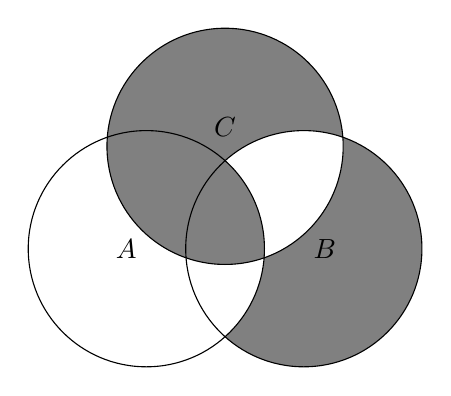
\begin{tikzpicture}
% Define circles for A, B, and C
\def\circleA{(-1,0) circle (1.5cm)}
\def\circleB{(1,0) circle (1.5cm)}
\def\circleC{(0,1.3) circle (1.5cm)}
% Shade B \ (A ∪ C)
\begin{scope}
\clip \circleB;
\fill[gray] \circleB;
\begin{scope}
\clip \circleA;
\fill[white] \circleA;
\end{scope}
\begin{scope}
\clip \circleC;
\fill[white] \circleC;
\end{scope}
\end{scope}
% Shade C \ B
\begin{scope}
\clip \circleC;
\fill[gray] \circleC;
\begin{scope}
\clip \circleB;
\fill[white] \circleB;
\end{scope}
\end{scope}
% Shade C ∩ A
\begin{scope}
\clip \circleC;
\clip \circleA;
\fill[gray] \circleA;
\end{scope}
% Outline the circles and label them
\draw \circleA node [text=black, left] {$A$};
\draw \circleB node [text=black, right] {$B$};
\draw \circleC node [text=black, above] {$C$};
\end{tikzpicture}

Below is the prove for  \textbf{15(c)}.
\begin{alignat*}{2}
x \in (A \triangle C) \triangle (A \cup B) &\equiv x \in A \triangle [C \triangle (A \cup B)] && \quad \textbf{(1)}\\
&\equiv x \in A \triangle [(A \cup B) \triangle C] && \quad \textbf{(2)}\\
&\equiv x \in [A \triangle (A \cup B)] \triangle C && \quad \textbf{(3)}\\
&\equiv x \in [(A \cup B) \triangle A] \triangle C && \quad \textbf{(4)}\\
&\equiv x \in [(A \triangle A) \triangle (B \setminus A)] \triangle C && \quad \textbf{(5)}\\
&\equiv x \in [\emptyset \triangle (B \setminus A)] \triangle C && \quad \textbf{(6)}\\
&\equiv x \in ([\emptyset \cup (B \setminus A)] \setminus [\emptyset \cap (B \setminus A)] ) \triangle C && \quad \textbf{(7)}\\
&\equiv x \in [(B \setminus A) \setminus \emptyset] \triangle C && \quad \textbf{(8)}\\
&\equiv x \in (B \setminus A) \triangle C && \quad \textbf{(9)}\\
\end{alignat*}

Below is the corresponding chain of justification for \textbf{Exercise 15(c)}.
\begin{alignat*}{2}
&\textbf{(1)} && \quad \text{\textbf{Exercise 12} Associative Law, RHS}\\
&\textbf{(2)} && \quad \text{\textbf{Exercise 14(c) Proof Line 3} Commutative Law}\\
&\textbf{(3)} && \quad \text{\textbf{Exercise 12} Associative Law}\\
&\textbf{(4)} && \quad \text{\textbf{Exercise 14(c) Proof Line 3} Commutative Law}\\
&\textbf{(5)} && \quad \text{\textbf{Exercise 14(a)} Result of Exercise}\\
&\textbf{(6)} && \quad A \triangle A \equiv (A \cup A) \setminus (A \cap A) \equiv A \setminus A \equiv \emptyset\\
&\textbf{(7)} && \quad \emptyset \cup X \equiv X \quad \text{and} \quad \emptyset \cap X \equiv \emptyset\\
&\textbf{(8)} && \quad X \setminus \emptyset \equiv X \wedge \neg \emptyset \equiv X \wedge U \equiv X \quad \text{, where $U$ is the universal set and $\neg \emptyset \equiv U$}\\
&\textbf{(9)} && \quad \text{LHS}\\
\end{alignat*}

\end{flushleft}	
\end{document}

